\chapter{Ferramentas}
\label{c.ferramentas}

\section{Unity}
\label{s.unity}
Tendo em vista que a aplicação será feita em um dispositivo com sistema operacional Android, a ferramenta de desenvolvimento escolhida deverá oferecer suporte para este tipo de dispositivo. A Google® oferece recursos para desenvolvimento em RV para Android e possui duas opções de ferramentas: SDK do Android, SDK do Unity, SDK do iOS e SDK do Unreal Engine 4. \cite{googledocumentacao} 

As opções contam com um projeto exemplo e materiais explicativos sobre o desenvolvimento de aplicações em realidade virtual. Além disso, a Google® oferece guias de boas práticas para a criação de aplicações em RV. 

Após análise, foi escolhido o SDK do Unity para o desenvolvimento da aplicação pois o mesmo oferece um ambiente gráfico intuitivo que não depende somente do código puro. Além disso, o Unity possibilita a exportação da aplicação para múltiplas plataformas de forma simples e rápida.

Segundo a empresa \citeonline{unitynumbers}, esta feramenta é o principal software de desenvolvimento de jogos em escala global com 5 bilhões de jogos feitos em Unity baixados no 3º semestre de 2016 e 770 milhões de pessoas que jogam jogos feitos com a ferramenta. Na área da RV, é estimado que 90\% dos jogos desenvolvidos para o Samsung Gear VR e 53\% dos jogos desenvolvidos para o Oculus Rift foram feitos através do Unity.

O ambiente de desenvolvimento do Unity pode ser visualizado na Figura X, onde o menu do lado esquerdo contém os objetos presentes na cena, o centro contém a cena em si e o lado direito as propriedades dos objetos selecionados. Esta disposição dos elementos pode ser personalizada pelo usuário. Em cada elemento da cena, é possível adicionar scripts que definirão as ações sobre os objetos, podendo ser decorrentes do input do usuário e do estado da aplicação em geral. O Unity utiliza duas linguagens de programação para a criação de scripts: C\# e UnityScript.  

\begin{figure}[h]
	\caption{\small Unity}
	\centering
	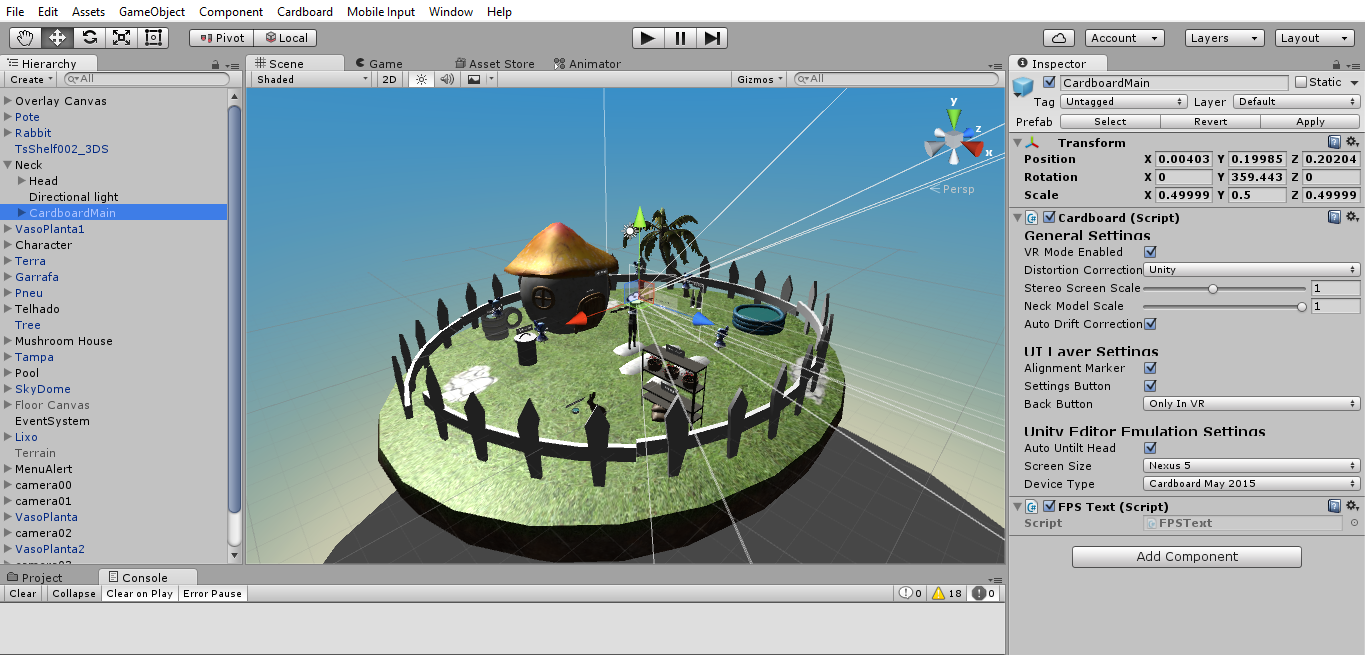
\includegraphics[height= 8cm]{Imagens/unity.png}
	\label{f.unity}
	\legend{\small Fonte: Elaborada pelo autor.}
\end{figure}

A fim de criar uma imagem para cada olho e proporcionar a sensação de imersão, são utilizadas duas câmeras (uma para cada olho). De acordo com a documentação oficial do Unity, para mover ou girar a câmera, é preciso anexar as mesmas à um objeto. Desta forma, ao movimentar o objeto, as câmeras refletirão o movimento. 

\subsection{Integração Unity e Google VR}
\label{ss.unitygoogle}

Para facilitar o desenvolvimento de aplicações para o Google Cardboard e o Daydream, o Unity possui integração nativa com o Google VR. Para recursos adicionais, a Google disponibiliza a Google VR SDK (Coleção de desenvolvimento de software) que requere a versão 5.2.1 ou superior do Unity e traz recursos como áudio espacial, suporte para o controle Daydream, ferramentas utilitárias e exemplos.  Segundo a \citeonline{googleunity}, a integração do Unity com o Google VR possibilita a localização da cabeça do usuário, renderização stereo, entre outros. 

\section{Capacetes de Visualização}
\label{s.capacetes}

Para este projeto, serão utilizados dois capacetes de visualização: o Google Cardboard (Figura X) e o VR Box (Figura X). Ambos foram escolhidos devido ao baixo custo e por utilizarem um smartphone como display. 

\begin{figure}[H]
	
	\begin{minipage}{.5\textwidth}{
			\centering
			\captionof{figure}{\small Google Cardboard}
			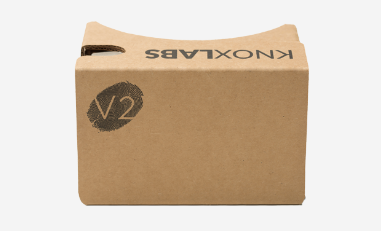
\includegraphics[height=4cm]{Imagens/googlecardboard.png}		
			\label{f.googlecardboard}	
			\legend{\small Fonte: \cite{googlecardboard}.}
		}
	\end{minipage}
	\begin{minipage}{.5\textwidth}{
			\centering
			\captionof{figure}{\small VR Box}
			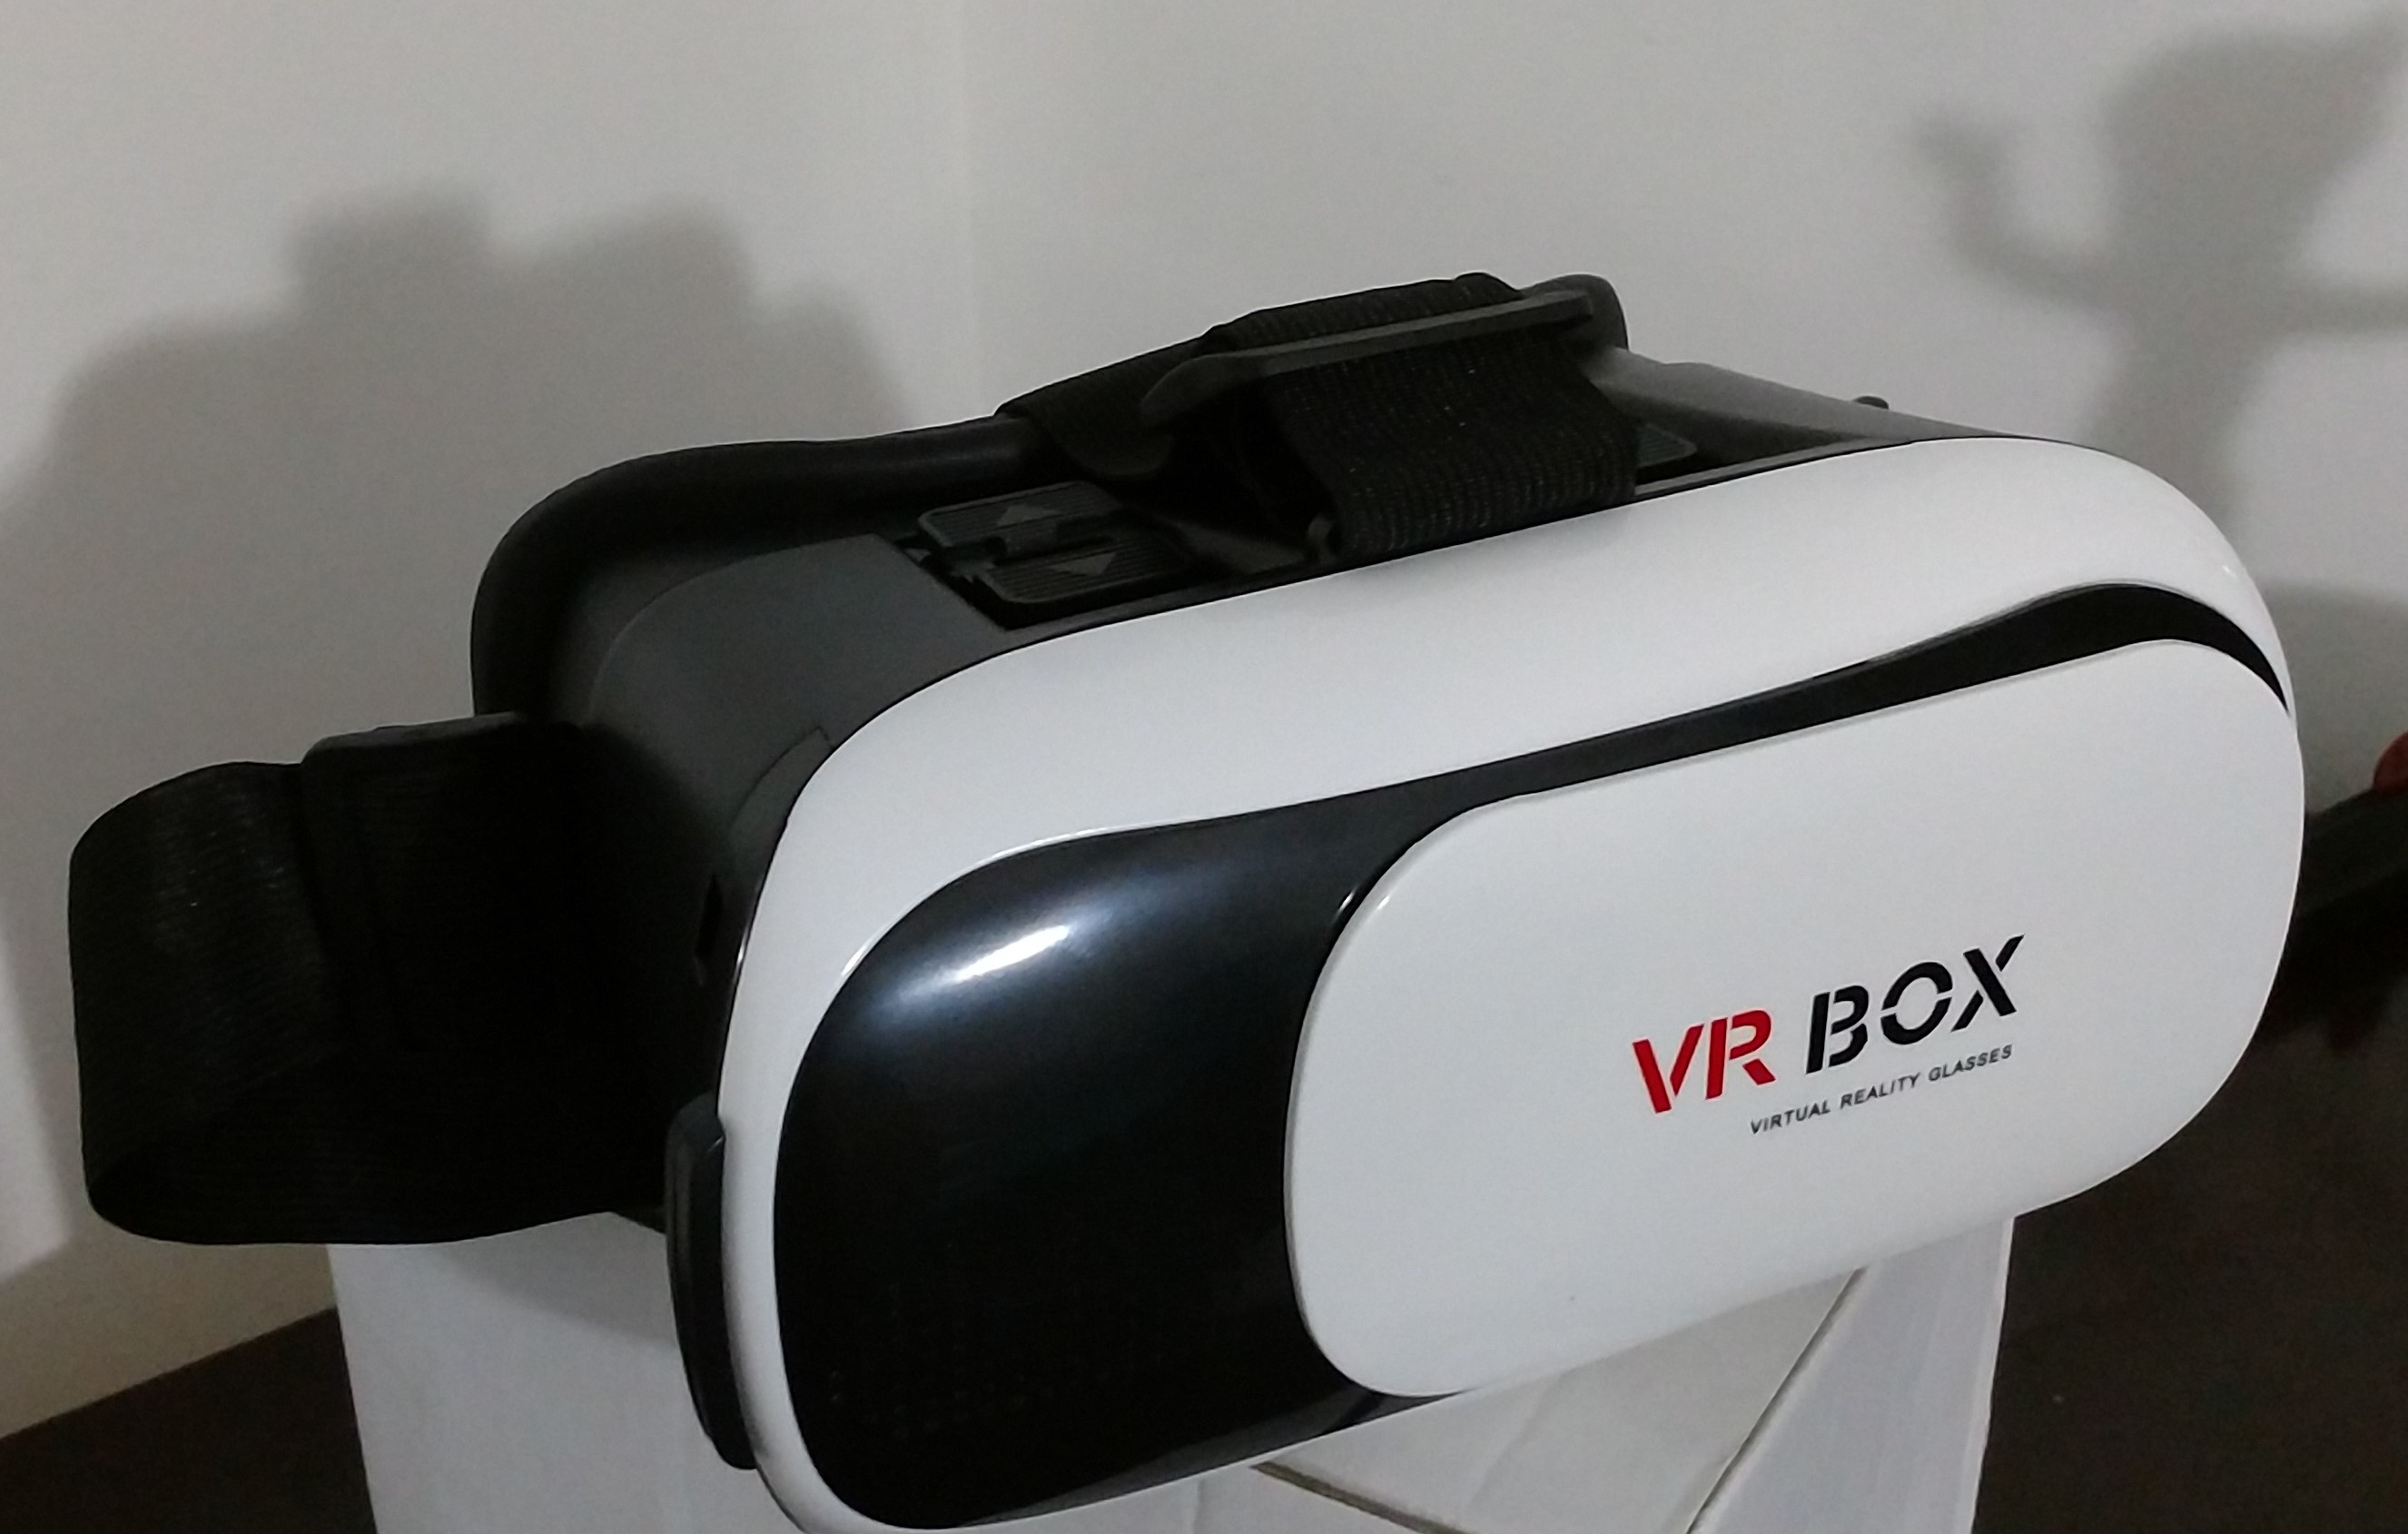
\includegraphics[height=4cm]{Imagens/vrbox.jpg}		
			\label{f.vrbox}
			\legend{\small Fonte: Elaborada pelo autor.}	
		}
	\end{minipage}
	
\end{figure}


O Google Cardboard proporciona experiências de imersão para todas as pessoas de uma forma simples e barata. Você pode montar seu próprio visualizador ou comprar um visualizador certificado com o selo “Funciona com o Google Cardboard” para ficar a apenas um passo de ter a realidade virtual no seu smartphone. \cite{googlecardboard}

O Google Cardboard 2.0 pode ser adquirido em diversos modelos como mostra a Figura X. Apesar da primeira versão do Cardboard possuir um modelo pra a montagem do visualizador, o modelo da segunda versão ainda não foi disponibilizado pela empresa, apesar de existir modelos de outras fontes.

\begin{figure}[h]
	\caption{\small Google Cardboard V2 Modelos}
	\centering
	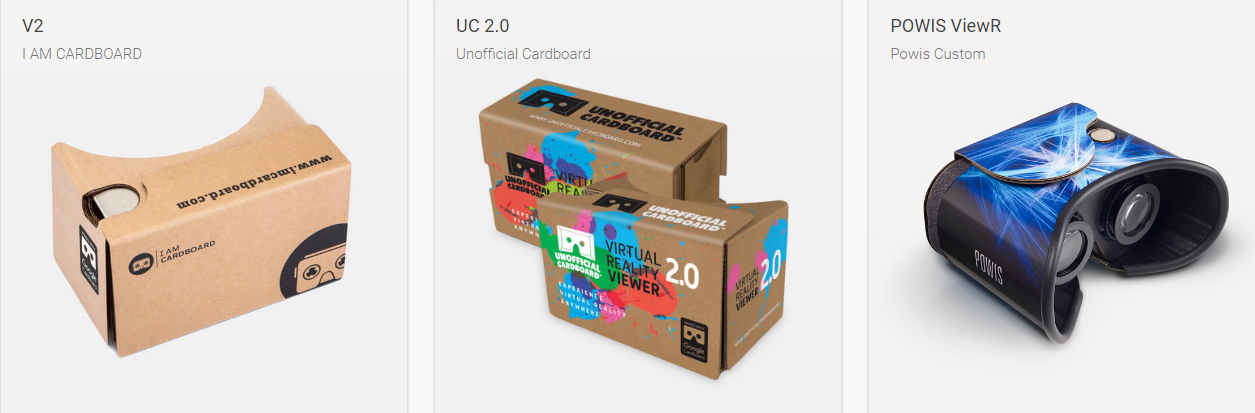
\includegraphics[scale=0.5]{Imagens/modelos.png}
	\label{f.modelos}
	\legend{\small Fonte: \cite{googlecardboard}.}
\end{figure}

Originalmente, o Google Cardboard não possui suporte para a fixação na cabeça do usuário, ou seja, o usuário terá que segurar o visualizador durante toda a experiência em RV, o que dificulta o uso de controle externos já que os mesmos deverão ser utilizados com somente uma das mãos do usuário. O visualizador comporta smartphones de 4.7 até 5.5 polegadas.

O visualizador VR Box vem acompanhado de um controle com comunicação Bluetooth além de já possuir o suporte para cabeça. Diferentemente do Google Cardboard, o VR Box possui um compartimento ajustável para a inserção do smartphone (Figura X), possibilitando uma melhor fixação de smartphones de diversos tamanhos (4,7 até 6 polegadas) ao visualizador.

\begin{figure}[H]
	\caption{\small Compartimento para smartphone}
	\centering
	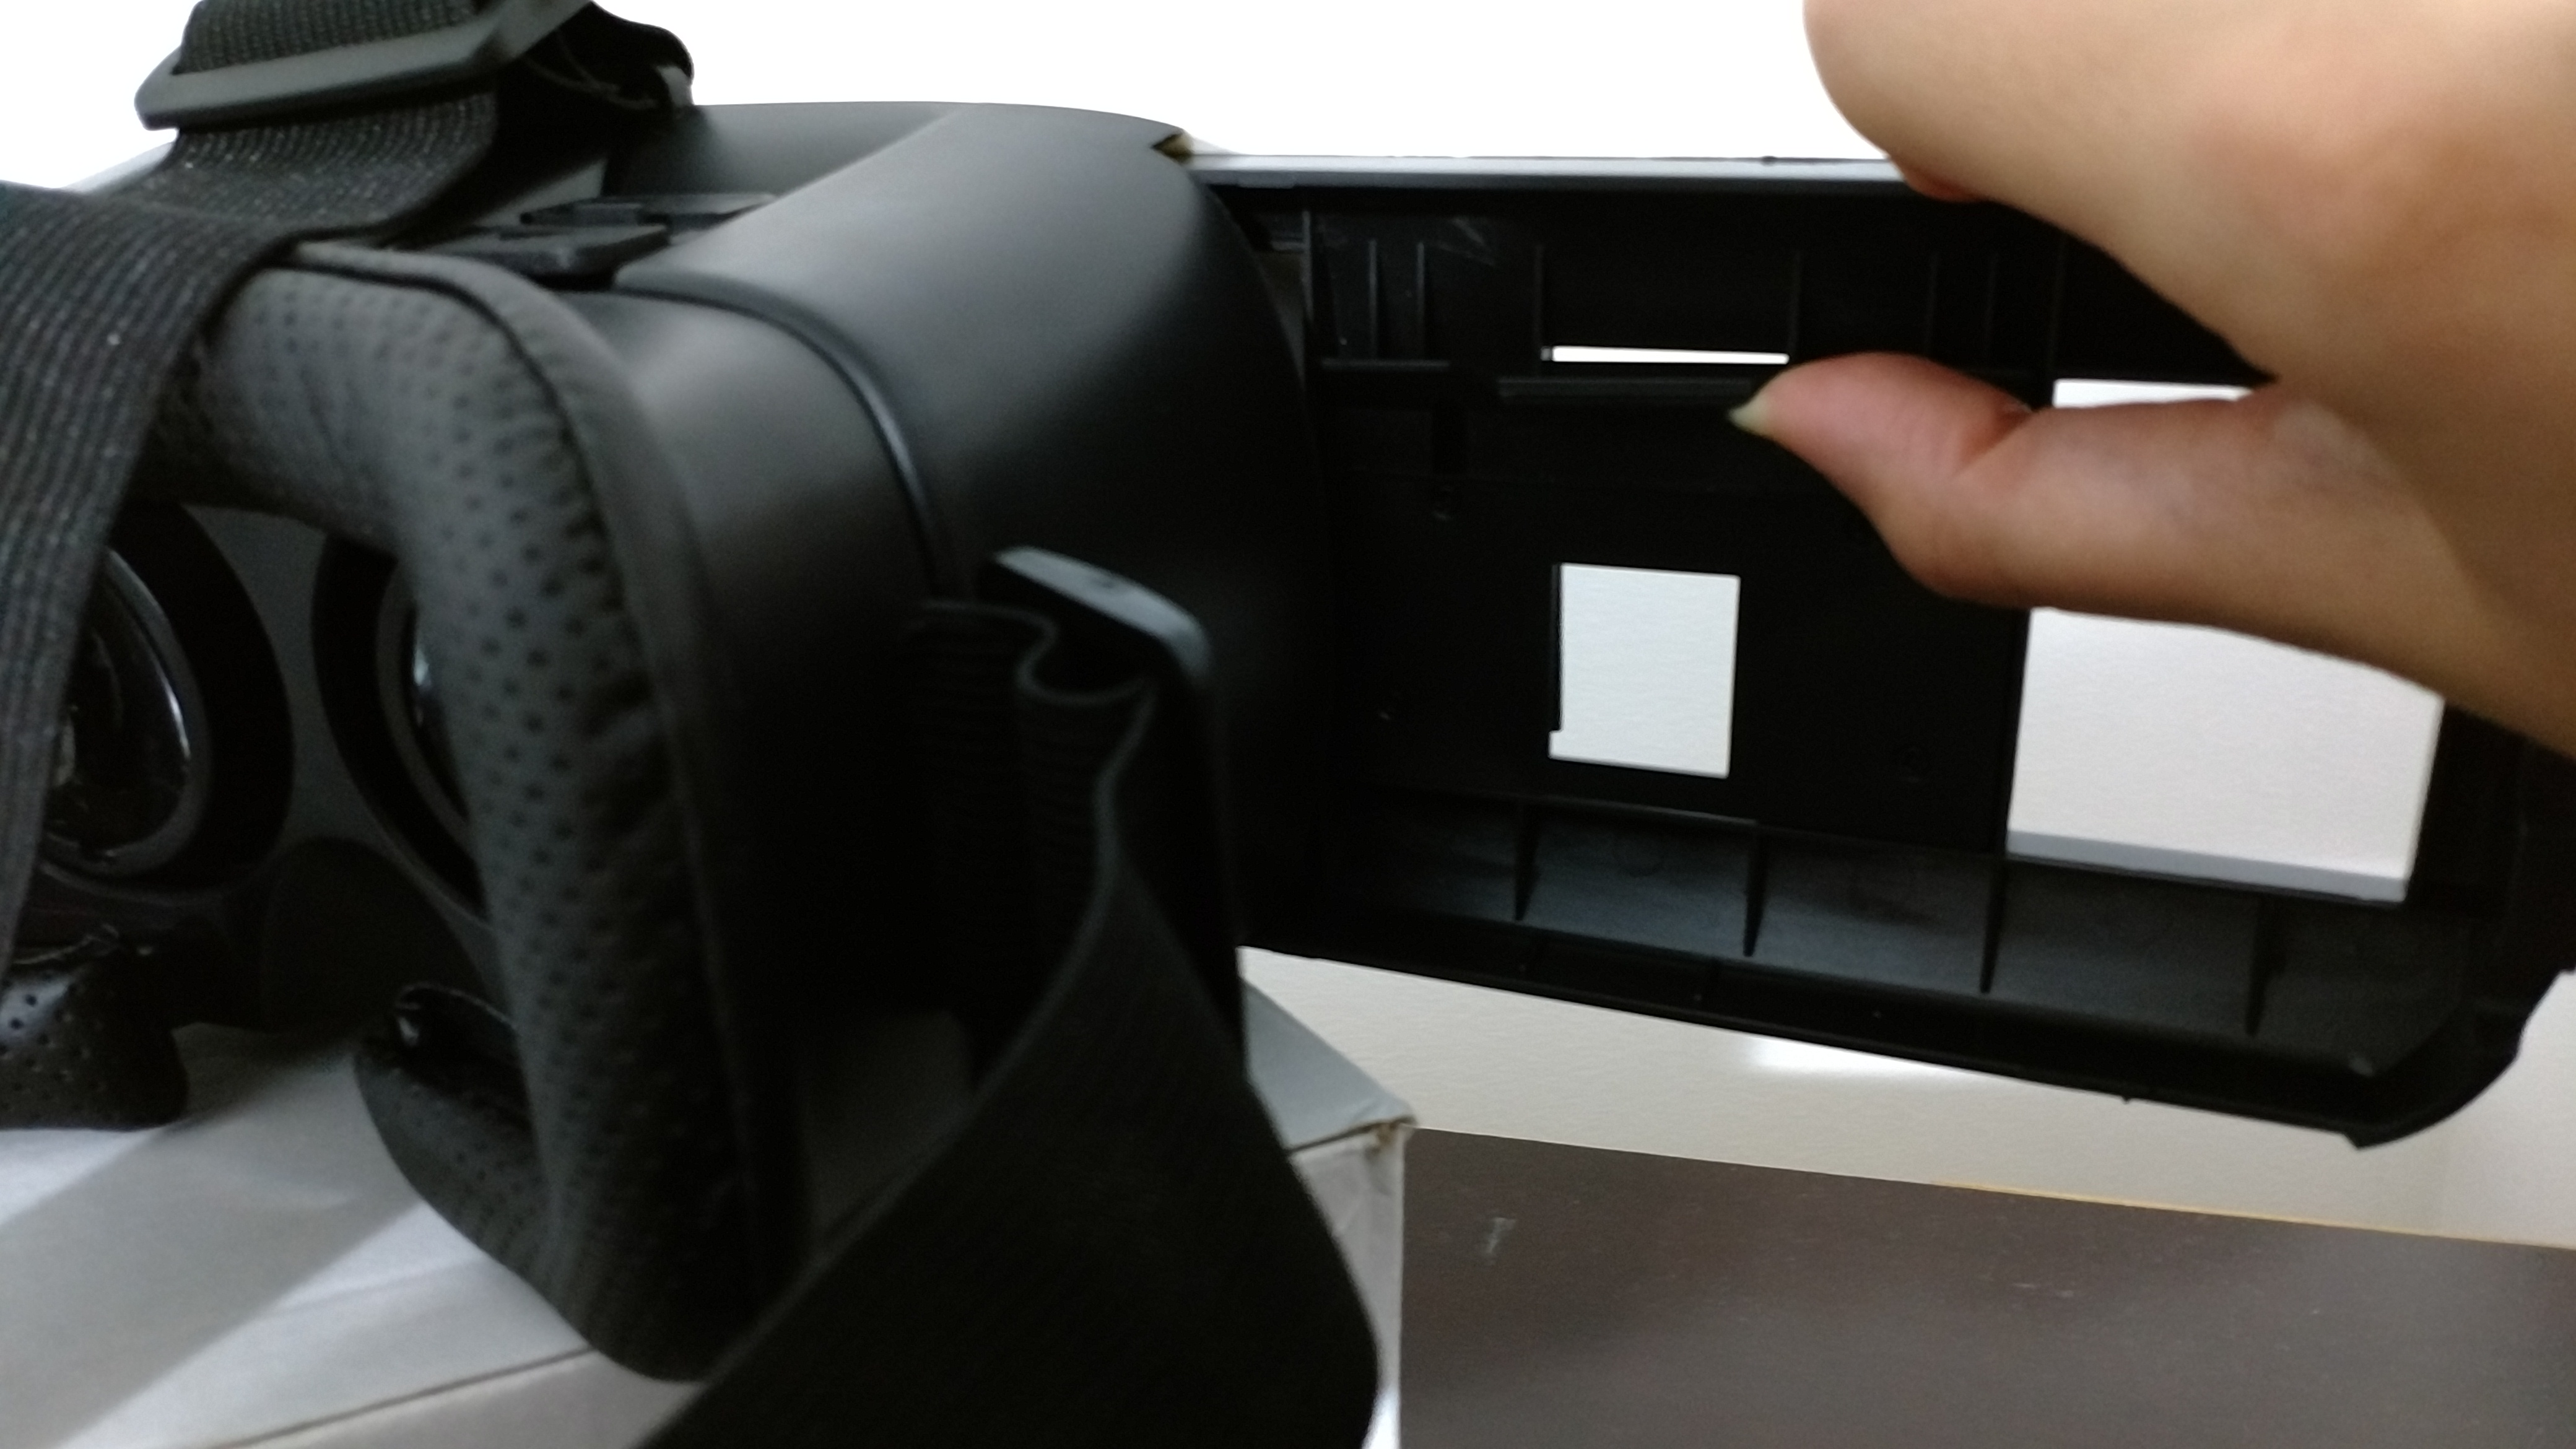
\includegraphics[height=5cm]{Imagens/extensor.jpg}
	\label{f.extensor}
	\legend{\small Fonte: Elaborada pelo autor.}
\end{figure}



\section{Dispositivo Móvel}
\label{s.dispositivomovel}

Para se obter uma experiência completa em RV, é necessário que o dispositivo móvel possua giroscópio e acelerômetro. Ao adquirir o Google Cardboard é necessário observar as especificações do visualizador para saber quais tamanhos de telas são suportadas. 

Os testes previstos neste projeto serão realizados em um smartphone da Motorola, modelo Moto Z. As especificações principais deste dispositivo podem ser visualizadas na Tabela X



